\section{Jao Gap}\label{sec:JaoGap}
A theoretical explanation for the Jao Gap (Figure \ref{fig:JaoGap}) comes from
\citet{van2012}, who propose that in a star directly above the transition mass,
due to asymmetric production and destruction of He$^{3}$ during the
proton-proton I chain (ppI), periodic luminosity variations can be induced.
This process is known as convective-kissing instability. Such a star will
descend the pre-main sequence with a radiative core; however, as the star
reaches the zero age main sequence (ZAMS) and as the core temperature exceeds
$7\times 10^{6}$ K, enough energy will be produced by the ppI chain that the
core becomes convective. At this point the star exists with both a convective
core and envelope, in addition to a thin, radiative, layer separating the two.
Subsequently, asymmetries in ppI affect the evolution of the star's convective
core.

\begin{figure}
	\centering
	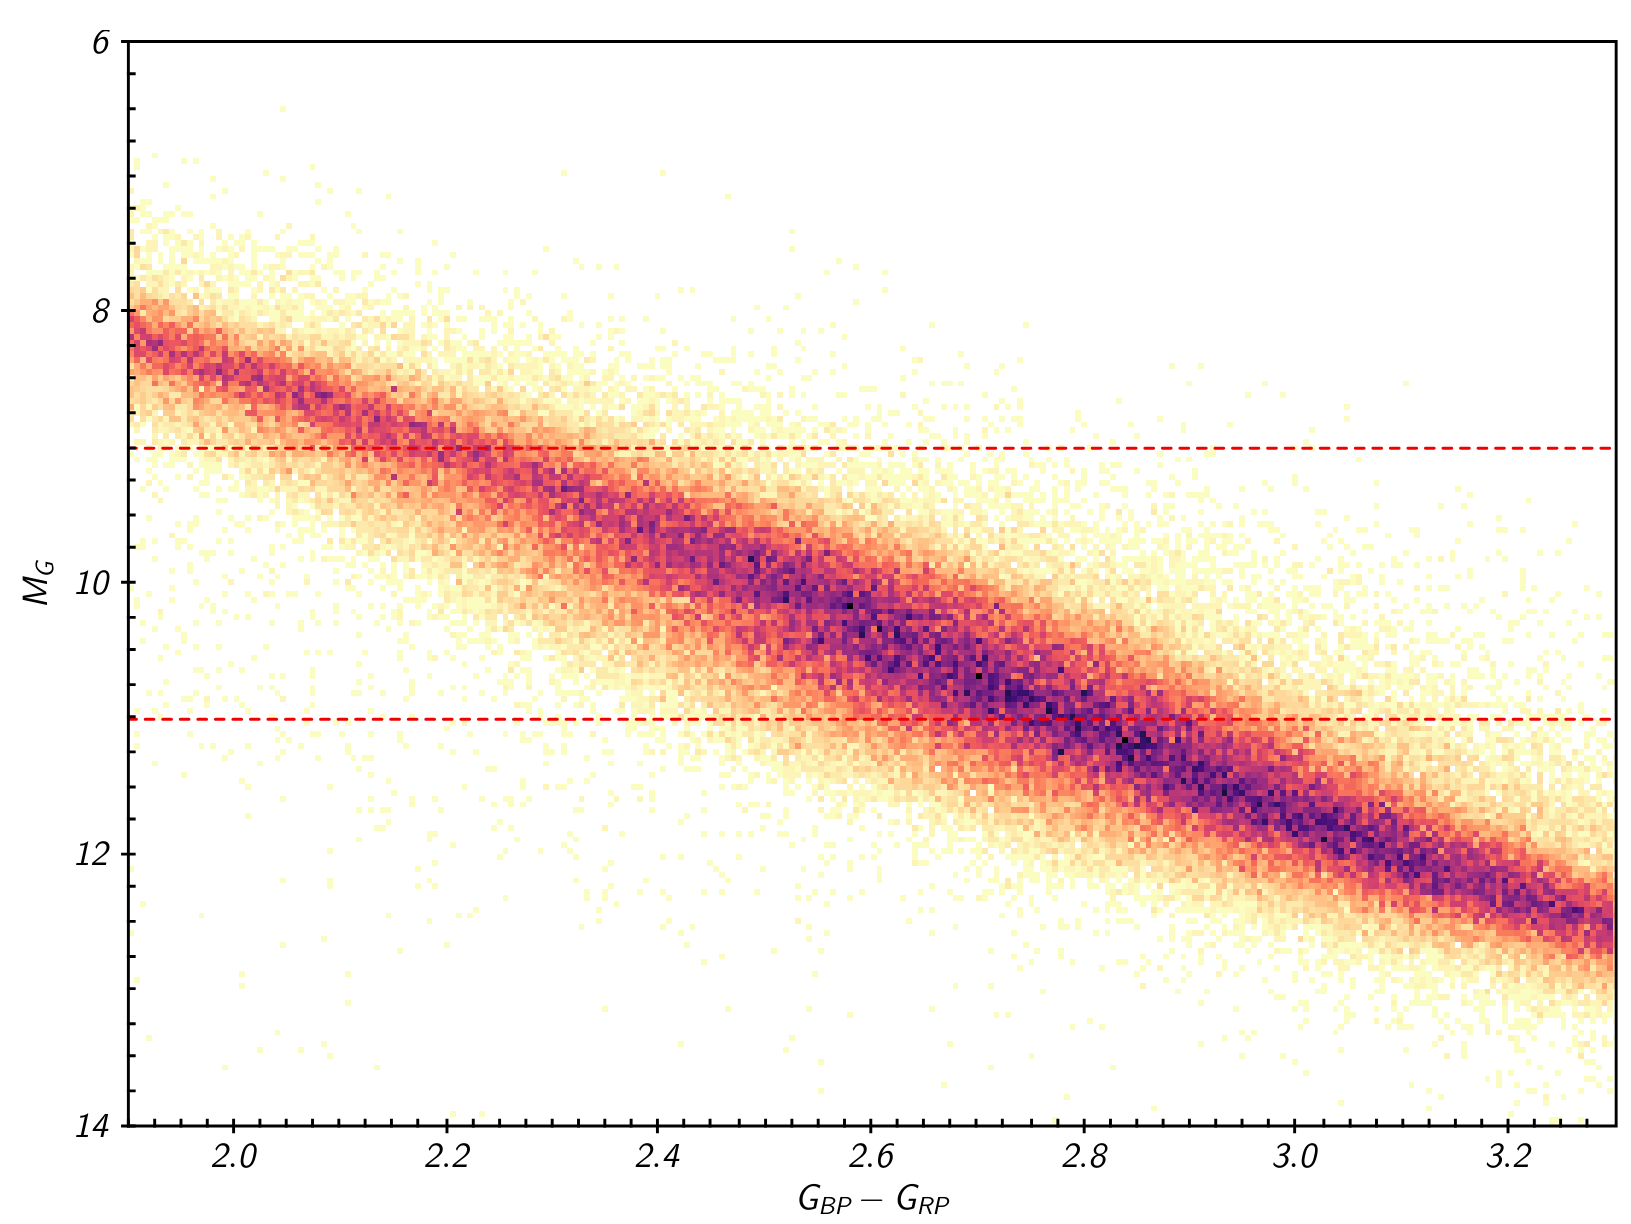
\includegraphics[width=0.45\textwidth]{src/figures/JaoGap.png}
	\caption{Figure 1 from \citet{Jao2018} showing the so called ``Jao Gap'' at
	$M_{G}\approx$ 10 {\color{red} [SHOULD I REMAKE THIS USING DR3 DATA?]}}
	\label{fig:JaoGap}
\end{figure}

The proton-proton I chain constitutes three reactions 
\begin{enumerate} 
	\item $p + p \longrightarrow d + e^{+} + \nu_{e}$
	\item $p + d \longrightarrow \ ^{3}\text{He} + \gamma$
	\item $^{3}\text{He} + ^{3}\text{He} \longrightarrow \ ^{3}\text{He} + 2p$ 
\end{enumerate} 
Because reaction 3 of ppI consumes $^{3}$He at a slower rate than it is
produced by reaction 2, core $^{3}$He abundance, and consequently the rate of
reaction 3, increases with time. The core convective zone expands as more of
the star becomes unstable to convection. This expansion continues until the
core connects with the convective envelope. At this point convective mixing can
transport material throughout the entire of the star and the high concentration
of $^{3}$He rapidly diffuses outward, away from the core, decreasing energy
generation as reaction 3 slows down. Ultimately, this leads to the convective
region around the core pulling back away from the convective envelope, leaving
in place the radiative transition zone, at which point $^{3}$He concentrations
grow in the core until it once again expands to meet the envelope.  These
periodic mixing events will contine until the $^{3}$He concentration throughout
the star reach an equlibtium ultimatly resulting in a fully convective star.
Figure \ref{fig:Kippenhan1} traces the evolution of a charecteristic star
within the Jao Gap's mass range.

\begin{figure*}
	\centering
	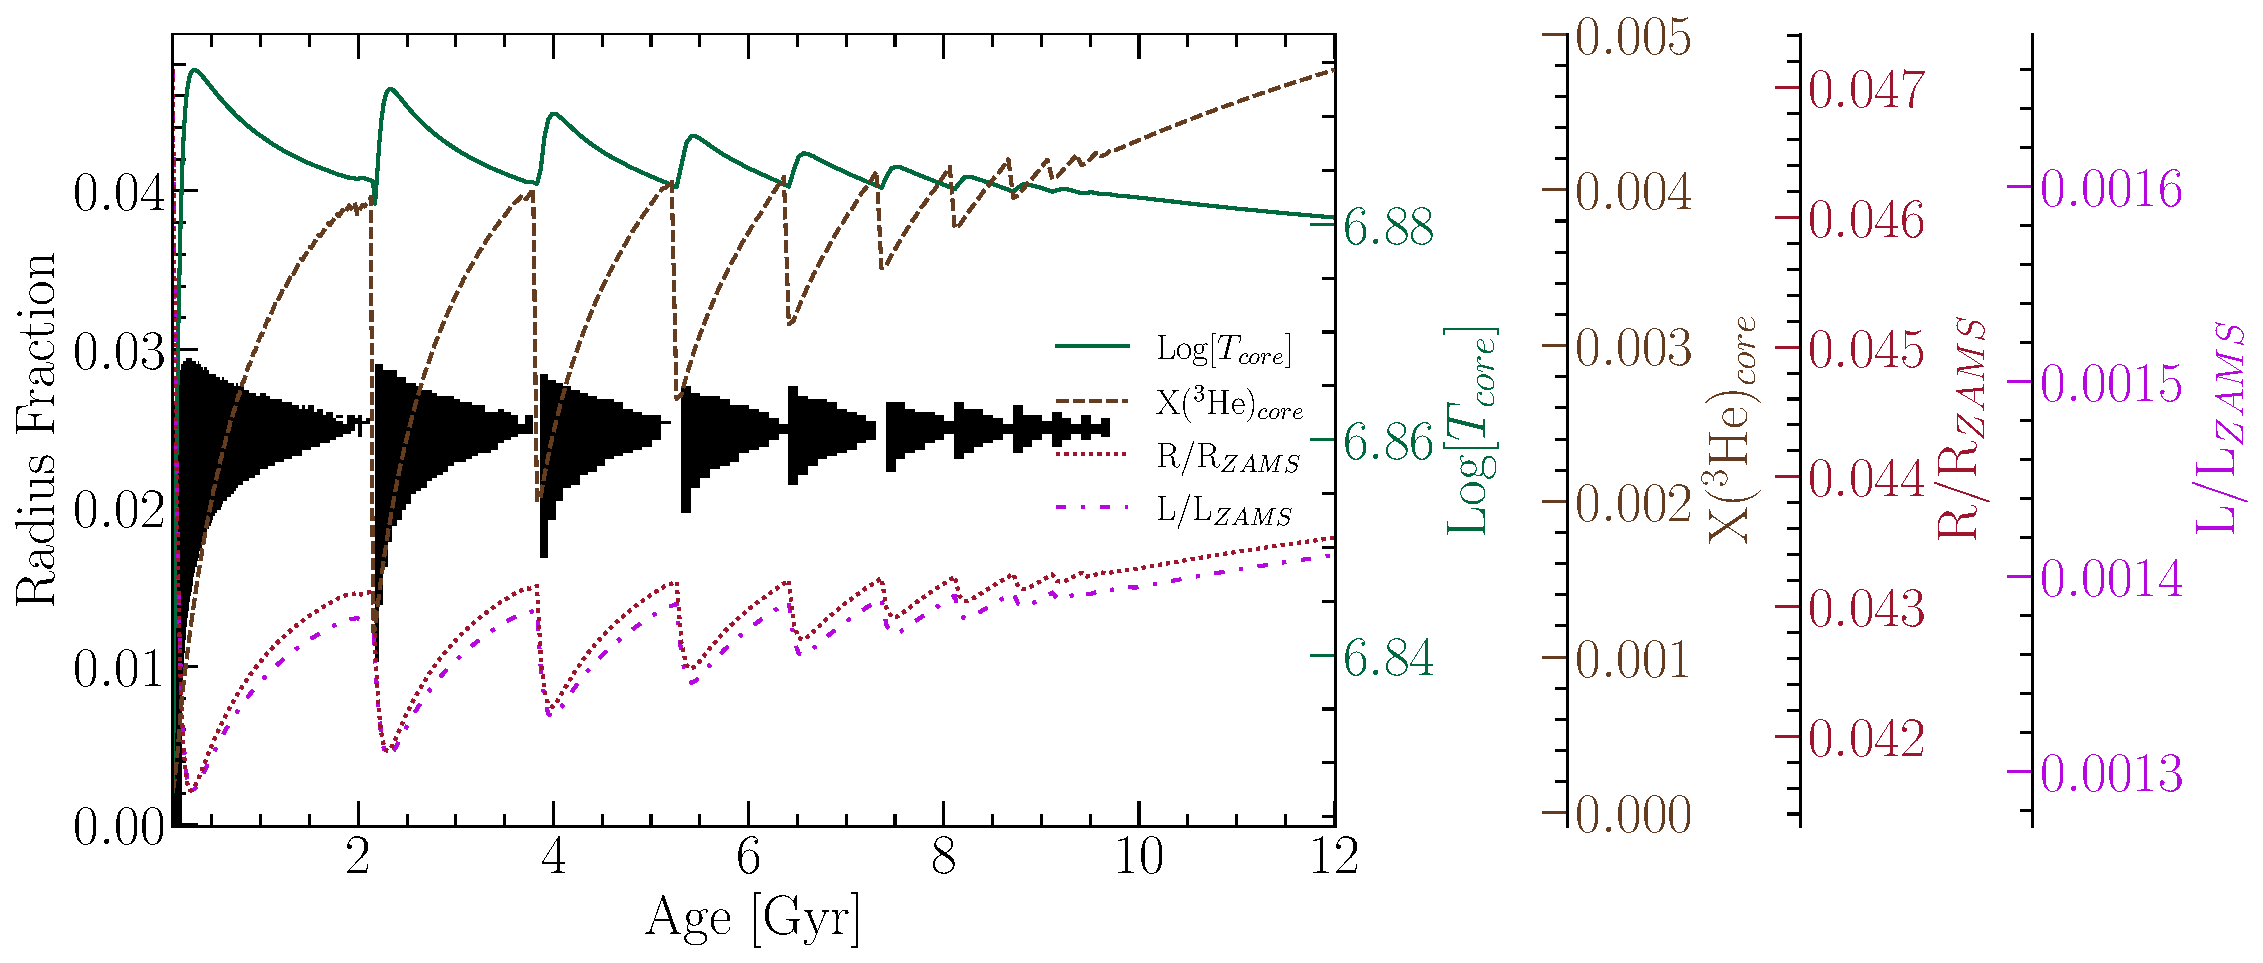
\includegraphics[width=0.95\textwidth]{src/figures/NotebookFigs/Kippenhan.pdf}
	\caption{Kippenhan diagram for a charectaristic stellar model of 0.35625
	$M_{\odot}$ which is within the Jao Gap's mass range. The black shaded
	regions denote whether, at a particular model age, a radial shell within
	the model is radiative or convective (with white meaning convective and
	black meaning radiative). The lines trace the models cote temperature, core
	$^{3}$He mass fraction, fractional luminosity wrt the zero age main
	sequence and fractional radius wrt. the zero age main sequence.}
	\label{fig:Kippenhan1}
\end{figure*}


\subsection{Efforts to Model the Gap}
Since the identification of the Gaia M-dwarf gap, stellar modeling has been
conducted to better constrain its location, effects, and exact cause.
Both \citet{Mansfield2021} and \citet{Feiden2021} identify that the gap's mass
location is correlated with model metallicity --- the mass-luminosity
discontinuity in lower metallicity models being at a commensurately lower mass.
\citet{Feiden2021} suggests this dependence is due to the steep relation of
the radiative temperature gradient, $\nabla_{rad}$, on temperature and in turn,
on stellar mass.

\begin{align}\label{eqn:radGrad}
	\nabla_{rad} \propto \frac{L\kappa}{T^{4}}
\end{align}

As metallicity decreases so does opacity, which, by Equation \ref{eqn:radGrad},
dramatically lowers the temperature where radiation will dominate energy transport
\citep{Chabrier1997}. Since main sequence stars are virialized the core
temperature is proportional to the core density and total mass (Equation
\ref{eqn:TMRelation}). Therefore, if the core temperature where
convective-kissing instability is expected decreases with metallicity, so too
will the mass of stars which experience such instabilities.

\begin{align}\label{eqn:TMRelation}
	T_{c} \propto \rho_{c}M^{2}
\end{align}

The strong opacity dependence of the Jao Gap begs the question: \textbf{what is
the affect of different opacity {\color{red} [estimates?]} on gap properties}.
As we can see above changing opacity should affect the gaps location in the
mass-luminosity relation and therefore in a color-magnitude diagram. Moreover,
current models of the gap have yet to locate it precisly in the CMD
\citep{Feiden2021} with an approximate {\color{red} [VALUE]} offset between the
observed and models gaps. 
